% standalone wrapper for a tikz picture
\documentclass[tikz,border=2pt]{standalone}
\usepackage{xcolor}
\usepackage{tikz}
\usetikzlibrary{shapes,arrows,positioning,shadows,patterns,arrows.meta,calc}
\definecolor{cwAlert}{RGB}{220,50,50}
\definecolor{cwFlow}{RGB}{50,120,220}
\definecolor{cwDecoy}{RGB}{120,180,50}
\definecolor{cwBorder}{RGB}{80,80,80}
\definecolor{ImperialBlue}{RGB}{0,62,116}
\definecolor{ImperialNavy}{RGB}{0,33,71}
\definecolor{ImperialLightBlue}{RGB}{155,203,235}
\begin{document}

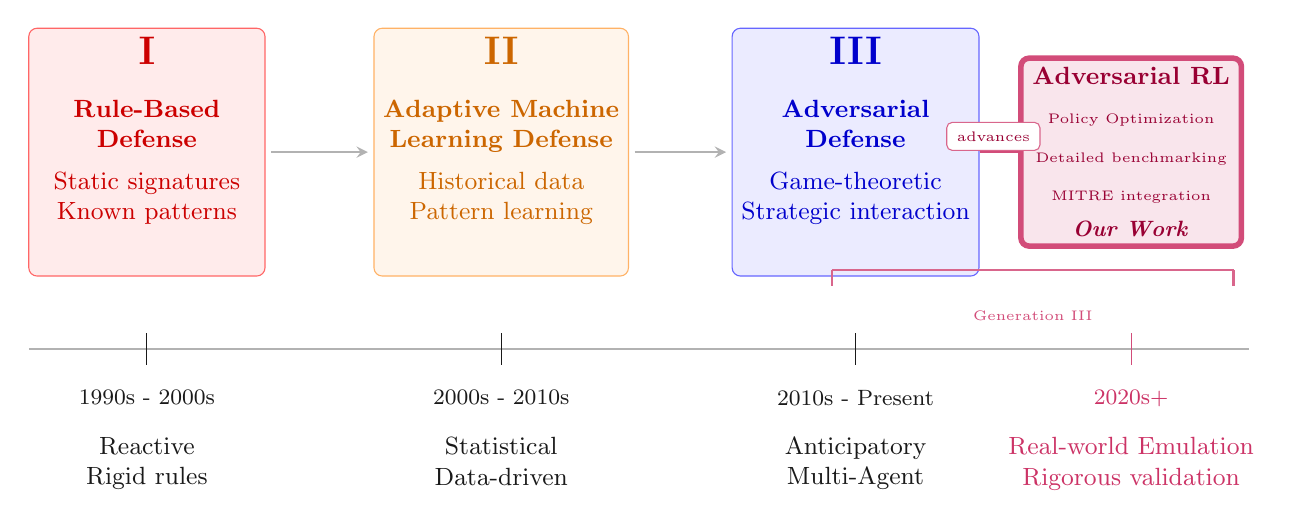
\begin{tikzpicture}[
    font=\small,
    generation/.style={
        draw=gray!40,
        fill=white,
        minimum width=3cm,
        minimum height=2.5cm,
        rounded corners=3pt,
        align=center
    },
    redaccent/.style={
        draw=red!60,
        fill=red!8,
        text=red!80!black
    },
    orangeaccent/.style={
        draw=orange!60,
        fill=orange!8,
        text=orange!80!black
    },
    blueaccent/.style={
        draw=blue!60,
        fill=blue!8,
        text=blue!80!black
    },
    ourwork/.style={
        draw=purple!70,
        fill=purple!10,
        minimum width=2.8cm,
        minimum height=2.3cm,
        rounded corners=3pt,
        align=center,
        line width=2pt,
        text=purple!80!black
    },
    arrow/.style={
        -stealth,
        thick,
        gray!60,
        shorten >=2pt,
        shorten <=2pt
    }
]
% Generation 1
\node[generation, redaccent] at (0,0) (g1) {
    {\Large \textbf{I}}\\[8pt]
    \textbf{Rule-Based}\\
    \textbf{Defense}\\[4pt]
    \small Static signatures\\
    \small Known patterns\\[6pt]
};
% Generation 2  
\node[generation, orangeaccent] at (4.5,0) (g2) {
    {\Large \textbf{II}}\\[8pt]
    \textbf{Adaptive Machine}\\
    \textbf{Learning Defense}\\[4pt]
    \small Historical data\\
    \small Pattern learning\\[6pt]
};
% Generation 3 - Updated to Adversarial
\node[generation, blueaccent] at (9,0) (g3) {
    {\Large \textbf{III}}\\[8pt]
    \textbf{Adversarial}\\
    \textbf{Defense}\\[4pt]
    \small Game-theoretic\\
    \small Strategic interaction\\[6pt]
};
% Our Work - Advanced approach within Gen 3
\node[ourwork] at (12.5,0) (ourwork) {
    \textbf{Adversarial RL}\\[3pt]
    \tiny  Policy Optimization\\[3pt]
    \tiny Detailed benchmarking\\[3pt]
    \tiny MITRE integration\\[2pt]
    \footnotesize \textbf{\textit{Our Work}}
};
% Evolution arrows
\draw[arrow] (g1.east) -- (g2.west);
\draw[arrow] (g2.east) -- (g3.west);
% Connection to our work (different style to show it's within Gen 3)
\draw[purple!70, thick] (g3.east) -- (ourwork.west);

% "Advances" in its own small box with text wrapping
\node[draw=purple!60, fill=white!5, rounded corners=2pt, 
      font=\tiny, text width=0.95cm, 
      align=center, text=purple!80!black] at (10.75,0.2) {advances
};
% Timeline
\draw[thick, black!30] (-1.5,-2.5) -- (14,-2.5);
% Timeline markers - Updated for three generations
\draw[black!90] (0,-2.3) -- (0,-2.7);
\node[below, black!90, font=\footnotesize] at (0,-2.9) {1990s - 2000s};
\draw[black!90] (4.5,-2.3) -- (4.5,-2.7);
\node[below, black!90, font=\footnotesize] at (4.5,-2.9) {2000s - 2010s};
\draw[black!90] (9,-2.3) -- (9,-2.7);
\node[below, black!90, font=\footnotesize] at (9,-2.9) {2010s - Present};

% Additional marker for our work (within the same era)
\draw[purple!70] (12.5,-2.3) -- (12.5,-2.7);
\node[below, purple!80, font=\footnotesize] at (12.5,-2.9) {2020s+};
% Key characteristics - Updated
\node[below, black!90, font=\small, align=center] at (0,-3.5) {
    Reactive\\
    Rigid rules
};
\node[below, black!90, font=\small, align=center] at (4.5,-3.5) {
    Statistical\\
    Data-driven
};
\node[below, black!90, font=\small, align=center] at (9,-3.5) {
    Anticipatory\\
    Multi-Agent
    
};
\node[below, purple!80, font=\small, align=center] at (12.5,-3.5) {
    Real-world Emulation\\
    Rigorous validation
};
% Bracket to show our work is within Gen 3
\draw[purple!60, thick] (8.7, -1.5) -- (13.8, -1.5);
\draw[purple!60, thick] (8.7, -1.5) -- (8.7, -1.7);
\draw[purple!60, thick] (13.8, -1.5) -- (13.8, -1.7);
\node[below, purple!70, font=\tiny] at (11.25, -1.9) {Generation III};
\end{tikzpicture}
\end{document}
